\documentclass[border=8pt]{standalone}
\usepackage{siunitx}\usepackage{xcolor}
\usepackage{tikz}\usetikzlibrary{arrows.meta,positioning}
\begin{document}
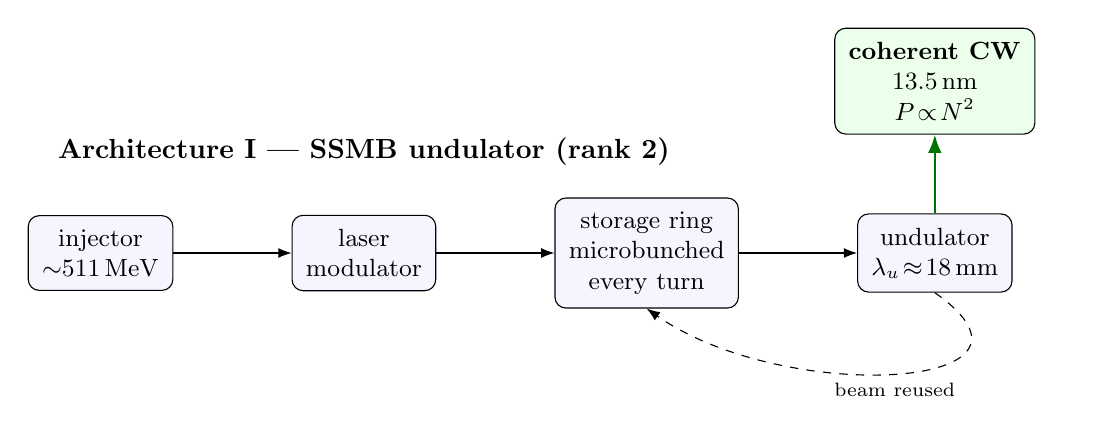
\begin{tikzpicture}[node distance=8mm and 15mm,every node/.style={font=\small},
  box/.style={draw,rounded corners,align=center,inner sep=5pt,minimum height=9mm,fill=blue!4},
  obox/.style={draw,rounded corners,align=center,inner sep=5pt,minimum height=9mm,fill=green!8}]
  \node[box] (gun) {injector\\$\sim$\SI{511}{\mega\electronvolt}};
  \node[box,right=of gun] (mod) {laser\\modulator};
  \node[box,right=of mod] (ring) {storage ring\\microbunched\\every turn};
  \node[box,right=of ring] (und) {undulator\\$\lambda_u\!\approx\!\SI{18}{\milli\meter}$};
  \node[obox,above=10mm of und] (o) {\textbf{coherent CW}\\\SI{13.5}{\nano\meter}\\$P\!\propto\!N^2$};
  \draw[-{Latex}] (gun)--(mod); \draw[-{Latex}] (mod)--(ring); \draw[-{Latex}] (ring)--(und);
  \draw[-{Latex},green!45!black,thick] (und)--(o);
  \draw[-{Latex},dashed] (und.south) to[out=-35,in=-35,looseness=1.5] node[below,font=\scriptsize]{beam reused} (ring.south);
  \node[font=\bfseries,above=1mm of mod,yshift=4mm] {Architecture I --- SSMB undulator (rank 2)};
\end{tikzpicture}
\end{document}
